\documentclass[notitlepage,letterpaper,12pt]{article} % para articulo

% Este es un comentario <- Los comentarios comienzan con % 
% todo lo que se escriba hasta el final de la linea será ignorado <- Este es otro comentario

%Lenguaje del documento
\usepackage[spanish]{babel} % silabea palabras castellanas <- Puedo poner comentarios para explicar de que va este comando en la misma línea

%Encoding
\usepackage[utf8]{inputenc} % Acepta caracteres en castellano
\usepackage[T1]{fontenc} % Encoding de salida al pdf

%Triunfó el mal
\usepackage[normalem]{ulem}
\useunder{\uline}{\ul}{}
\providecommand{\e}[1]{\ensuremath{\times 10^{#1}}}

\usepackage{aas_macros}

\usepackage{textcomp}
\usepackage{gensymb}


%Hipertexto
\usepackage[colorlinks=true,urlcolor=blue,linkcolor=blue]{hyperref} % navega por el doc: hipertexto y links

%Aquello de las urls
\usepackage{url} 

%simbolos matemáticos
\usepackage{amsmath}
\usepackage{amsfonts}
\usepackage{amssymb}
\usepackage{physics} 

% permite insertar gráficos, imágenes y figuras, en pdf o en eps
\usepackage{graphicx}
\usepackage{epstopdf}
\usepackage{multirow}
\usepackage{float}
\usepackage[export]{adjustbox}
% geometría del documento, encabezados y pies de páginas, márgenes
\usepackage{geometry}
\usepackage{comment}
\geometry{letterpaper}       % ... o a4paper o a5paper o ... 
\usepackage{fancyhdr} % encabezados y pies de pg
\pagestyle{fancy}
\chead{\bfseries {}}
\lhead{} % si se omite coloca el nombre de la seccion
%\rhead{fecha del doc}
\lfoot{\it Corrección parcial.}
\cfoot{ }
\rfoot{Universidad de los Andes}
%\rfoot{\thepage}
%margenes
\voffset = -0.25in
\textheight = 8.0in
\textwidth = 6.5in
\oddsidemargin = 0.in
\headheight = 20pt
\headwidth = 6.5in
\renewcommand{\headrulewidth}{0.5pt}
\renewcommand{\footrulewidth}{0,5pt}

\begin{document}
\title{Cúmulos abiertos: corrección parcial}
\author{
\textbf{Javier Alejandro Acevedo Barroso\thanks{e-mail: \texttt{ja.acevedo12@uniandes.edu.co}}}\\
\textit{Universidad de los Andes, Bogotá, Colombia}\\
} % Hasta aquí llega el bloque "author" (son dos autores por informe, orden alfabético)

%\date{Versión $\alpha \beta$ fecha del documento}
\maketitle %Genera el título del documento


%Resumen

%\begin{abstract}

%Usando un generador de señales 	CFG253 como fuente de voltaje en el circuito requerido de la practica, se observo la señal que produce un circuito RLC en un osciloscopio, con el objetivo de estudiar su resonancia eléctrica mediante la curva generada a partir de graficar el voltaje en la resistencia vs la frecuencia de oscilacion dada por la fuente  


 
%\end{abstract}

%Introducción

\section{Primer punto}
Hay un sistema estelar triple. ¿cuánto debe ser la magnitud de la una de las estrellas para que la magnitud total sea dos veces la magnitud del sistema si solo tuviera las otras dos estrellas?

Nombremos las magnitudes de las estrellas: m1, m2, m3.
La magnitud del sistema si solo estuvieran la estrella 1 y 2 se puede calcular usando las ecuaciones:
\begin{equation}
m_i = -2.5 \log(\frac{F_i}{F_0}).
\end{equation}
Donde $F_i$ es el flujo de la estrella $i$.
\begin{equation}
F_i = F_0 10^{-2m_i/5}.
\end{equation}
Entonces la magnitud del sistema 1,2 estará dada por:
\begin{equation}
m_{1,2} = -2.5 \log(\frac{F_1 + F_2}{F_0}).
\end{equation}
Y la magnitud del sistema triple por:
\begin{equation}
m_{T} = -2.5 \log(\frac{F_1 + F_2 + F_3}{F_0}).
\end{equation}
Aplicando la condición $m_T = 2m_{1,2}$:
\begin{equation}
2\log(\frac{F_1 + F_2}{F_0}) = \log(\frac{F_1 + F_2 + F_3}{F_0}),
\end{equation}
\begin{equation}
\log(\left(\frac{F_1+F_2}{F_0}\right)^2) = \log(\frac{F_1 + F_2 + F_3}{F_0}).
\end{equation}
De lo que se puede obtener:
\begin{equation}
(10^{-2m_1/5}+10^{-2m_2/5})^2 = 10^{-2m_1/5}+10^{-2m_2/5} + 10^{-2m_3/5}.
\end{equation}
Y despejar $m_3$:
\begin{equation}
m_3 = -2.5\log( (10^{-2m_1/5}+10^{-2m_2/5})^2 - 10^{-2m_1/5} - 10^{-2m_2/5} ).
\end{equation}
Entonces, la condición sera:
\begin{equation}
(10^{-2m_1/5}+10^{-2m_2/5})^2 - (10^{-2m_1/5} + 10^{-2m_2/5}) > 0,
\end{equation}

\begin{equation}
(10^{-2m_1/5}+10^{-2m_2/5})((10^{-2m_1/5} + 10^{-2m_2/5})-1) > 0,
\end{equation}
dado que $(10^{-2m_1/5}+10^{-2m_2/5})$ siempre será mayor que cero, la condición se resume a:
\begin{equation}
10^{-2m_1/5} + 10^{-2m_2/5} >1
\end{equation}

\section{Punto 2}
Una estrella super gigante azul de más de 39000K de temperatura superficial efectiva se detecta con una magnitud V=28.
\begin{itemize}
\item[a)] Suponga que no hay extinción ¿A qué distancia está la estrella?
\item[b)] Repita el cálculo anterior considerando ahora que el medio interestelar absorbe radiación en el visual en una magnitud de 0.8.
\end{itemize}

Asumiendo que no hay extinción, la distancia a la estrella está dada por el módulo de distancia $\mu = m-M$.
\begin{equation}
\mu = 5\log(r) - 5.
\end{equation}
Donde $r$ es la distancia a la estrella en parsecs.
Se puede despejar que:
\begin{equation}
r = 10^{(\mu +5)/5}.
\end{equation}
Por último, para calcular la distancia es necesario conocer la magnitud absoluta de la estrella.
Conociendo la temperatura de la estrella, nos podemos referir catálogos de tipos espectrales para estimar cual sería su magnitud absoluta.
Usando el catálogo del parcial:
\begin{table}[h!]
\centering
\begin{tabular}{|l|l|l|}
\hline
Spectral type & T(K) & M$_v$ \\ \hline
O5 & 40900 & -6.5  \\ \hline 
O6 & 38500 & -6.5  \\ \hline 
O7 & 36200 & -6.6  \\ \hline 
\end{tabular}
\caption{Número de colisiones a diferentes distancias en cinco minutos.}
\label{tiempoFijo}
\end{table}
\newpage
Usando una interpolación de primer, segundo y tercer orden, se obtiene casi los mismos resultados M$_v$ = -$6.5$.

Por lo tanto, el módulo de distancia será: $\mu = 28-(-6.5) = 34.5$, y la distancia a la estrella será $r = 79.43$ Mpc:


Para el caso con extinción se tiene las siguientes relaciones:
\begin{equation}
\mu = 5\log(r) - 5 + A_v,
\end{equation}
\begin{equation}
r = 10^{(\mu+5-A_v)/5}.
\end{equation}
Dado $A_v = 0.8$, la distancia será $r = 54.95$ Mpc

\section{Punto 3}
Observación en infrarojo ¿Por qué el cielo varía fuertemente al observar en JHK$_\text{s}$L?.

A continuación una representación visual de la respuesta de los filtros en función de la longitud de onda:


\begin{figure}[h]
  \centering
   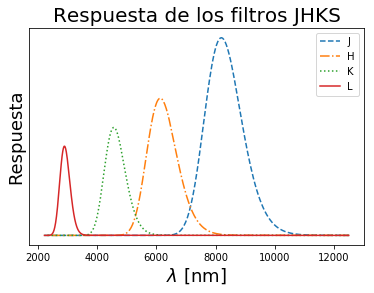
\includegraphics[scale= 0.8]{respuestaJHKS.png}
\end{figure}

%\bibliographystyle{unsrt} % estilo de las referencias 
%\bibliography{bibTes.bib} %archivo con los datos de los artículos citados

Se observa un pequeño hueco entre K y L.
La temperatura promedio de la atmósfera es de 15°C.
Usando la ley de Wien, se puede obtener el pico de emisión de cuerpo negro para una temperatura dada:
\begin{equation}
\lambda_{\text{max}} = b/T,
\end{equation}
con $b = 2897773$ [nm/K]. Por lo tanto, para la temperatura de la atmósfera, el pico de emisión será en $\lambda_m = 10056$ nm.

Por otro lado, la atmósfera no tiene una única temperatura, sino que al cambiar la altura también cambia la temperatura.
Estas temperaturas van desde 190K para las alturas cercanas a los 100km, hasta 290K para alturas bajas.
En términos de picos de emisión, esto implica un rango de 9986 a 15251 nm, por lo tanto, los picos de emisión no coinciden con las bandas de interés.
Sin embargo, el espectro de cuerpo negro incluye emisión en todo el espectro, y los picos implican que las regiones de interés sí son afectadas considerablemente.
Si además se incluye que la temperatura está variando con la altura, ya no se tendrá un espectro de cuerpo negro, sino una superposición de cuerpo negro que lleva a un ruido irregular en las bandas de interés.
Adicionalmente, la temperatura de las diferentes capas atmosféricas varia con la hora y época del año, de forma que corregir su contribución con total exactitud se vuelve imposible.

Por último, el espectro de emisión de la atmósfera no será simplemente un espectro de cuerpo negro, sino que incluirá picos de emisión en las líneas espectrales de las moléculas que la componen.
Gracias a las reglas de selección de la mecánica cuántica, las moléculas diatómica no emiten en el infrarojo. Lo anterior nos permite ignorar algunos de los principales componentes de la atmósfera, como el nitrógeno (N$_2$) y el oxígeno (O$_2$).
Dada su gran abundancia, la mayor parte de la emisión en infrarojo de la atmósfera se originará a partir de vapor de agua H$_2$O y dióxido de carbono (CO$_2$).
Sin embargo, hay una región del espectro (desde $~500$ nm a $~780$ nm) en donde prácticamente no hay emisión del agua, por lo que la transmitancia atmosférica sube y se ve limitada solo por las pocas líneas de emisión del CO$_2$ y el Ozono (O$_3$); que al no ser tan abundantes en la atmósfera, solo reducen levemente la transmitancia (como se observa en la imagen del punto 4 del parcial).

Concluendo, la emisión espectral de la atmósfera varía con el día y la temporada del año debido a los cambios de temperatura que sufre, además que las diferentes capas tienen diferentes temperaturas. Simultáneamente, la alta abundancia de agua, CO$_2$ y ozono en la atmósfera aumenta considerablemente el ruido atmosférico en infrarojo.
%\bibliography{mybib.bib} %archivo con los datos de los artículos citados

% Forma Manual de hacer las referencias
% Se escribe todo a mano...
% Descomentar y jugar

%\begin{thebibliography}{99}
%\bibitem{Narasimhan1993}Narasimhan, M.N.L., (1993), \textit{Principles of
%Continuum Mechanics}, (John Willey, New York) p. 510.

%\bibitem{Demianski1985}Demia\'{n}ski M., (1985), \textit{Relativistic
%Astrophysics,} in International Series in Natural Philosophy, Vol 110, Edited
%by \textit{D. Ter Haar}, (Pergamon Press, Oxford).
%\end{thebibliography}


%Fin del documento
\end{document}


Así mismo, el factor de calidad $Q$ está dado por:
\begin{equation}
Q = \frac{1}{R} \sqrt\frac{L}{C}
\end{equation}
Por lo tanto, el valor del factor de calidad

%Todo lo que escriba aquí será ignorado, aunque no fuera un comentario...
\begin{table}[h!]
\centering
\begin{tabular}{|l|l|l|}
\hline
2 cm   & 4 cm   & 8 cm   \\ \hline
175,77 & 129,77 & 88,77  \\ \hline
223,77 & 129,77 & 114,77 \\ \hline
219,77 & 134,77 & 77,77  \\ \hline
190,77 & 120,77 & 83,77  \\ \hline
\end{tabular}
\caption{Número de colisiones a diferentes distancias en cinco minutos.}
\label{tiempoFijo}
\end{table}

\begin{figure}[h]
  \centering
   \includegraphics[scale= 0.8]{jairos.png}
  \caption{Gráfica del periodo de la pulsación para diferentes razones entre las frecuencias naturales utilizando una pesa de 200g. Es de resaltar que el pico no está centrado en 1 pero está bastante cerca. Esto probablemente se debe a errores a la hora de medir la longitud de los péndulos.}
  \label{fig: cobre}
\end{figure}
